\section{СТРУКТУРНЫЕ ПАТТЕРНЫ}

В структурных паттернах рассматривается вопрос о том, как из классов и объектов
образуются более крупные структуры.

\textbf{Структурные паттерны уровня класса} используют наследование для составления
композиций из интерфейсов и реализаций.

\begin{itemize}
\item
\textit{Использование множественного наследования} для объединения нескольких классов в один.
В результате получается класс, обладающий свойствами всех своих родителей.
Особенно полезен этот паттерн, когда нужно организовать совместную работу
нескольких независимо разработанных библиотек.

\item
\textit{<<Адаптер>>}. В общем случае адаптер делает интерфейс одного класса (адаптируемого) 
совместимым с интерфейсом другого, обеспечивая тем самым унифицированную абстракцию
разнородных интерфейсов. Это достигается за счет закрытого наследования адаптируемому
классу. После этого адаптер выражает свой интерфейс в терминах операций адаптируемого класса.
\end{itemize}

Вместо композиции интерфейсов или реализаций \textbf{структурные паттерны уровня объекта}
компонуют объекты для получения новой функциональности.

\begin{itemize}
\item
\textit{<<Компоновщик>>}. Он описывает построение иерархии классов для
двух видов объектов: примитивных и составных.
Последние позволяют создавать произвольно сложные структуры из примитивных и
других составных объектов.

\item
\textit{<<Заместитель>>}. В этом паттерне объект берет на себя функции другого объекта.
У <<заместителя>> есть много применений.
Он может действовать как локальный представитель объекта, находящегося в
удаленном адресном пространстве. Или представлять большой объект,
загружаемый по требованию. Или ограничивать доступ к критически важному
объекту. <<Заместитель>> вводит дополнительный косвенный уровень доступа к
отдельным свойствам объекта. Поэтому он может ограничивать, расширять или
изменять эти свойства.

\item
\textit{<<Приспособленец>>} определяет структуру для совместного использования объектов.
Владельцы разделяют объекты, по меньшей мере, по двум причинам: для достижения эффективности
и непротиворечивости. 
Приспособленец акцентирует внимание на эффективности использования памяти.
В приложениях, в которых участвует очень много объектов, должны снижаться накладные
расходы на хранение. Значительной экономии можно добиться за счет разделения
объектов вместо их дублирования. Но объект может быть разделяемым, только
если его состояние не зависит от контекста. У объектов-приспособленцев такой
зависимости нет. Любая дополнительная информация передается им по мере необходимости.
В отсутствие контекстных зависимостей объекты-приспособленцы могут легко разделяться.

\item
\textit{<<Фасад>>} показывает, как один объект может представлять целую
подсистему. Фасад представляет набор объектов и выполняет свои функции, перенаправляя
сообщения объектам, которых он представляет. 

\item
\textit{<<Мост>>} отделяет абстракцию объекта от его реализации,
так что их можно изменять независимо.

\item
\textit{<<Декоратор>>} описывает динамическое добавление объектам новых обязанностей.
Это структурный паттерн, который рекурсивно компонует объекты с целью реализации
заранее неизвестного числа дополнительных функций.

\end{itemize}

Многие структурные паттерны в той или иной мере связаны друг с другом.

\pagebreak

\section{СТРУКТУРНЫЙ ПАТТЕРН \\ <<ПРИСПОСОБЛЕНЕЦ>>}

Паттерн <<приспособленец>> (Flyweight) использует разделение для эффективной поддержки
множества мелких объектов.

Паттерн <<приспособленец>> часто используется в сочетании с компоновщиком
для реализации иерархической структуры в виде ациклического направленного
графа с разделяемыми листовыми вершинами.

Часто наилучшим способом реализации объектов состояния и стратегии 
является паттерн <<приспособленец>>.

Например, в большинстве редакторов документов имеются средства форматирования и
редактирования текстов, в той или иной степени модульные.
Объектно-ориентированные редакторы обычно применяют объекты для представления
таких встроенных элементов, как таблицы и рисунки.
Но они не используют объекты для представления каждого символа, несмотря на то что
это увеличило бы гибкость на самых нижних уровнях приложения.
Ведь тогда к рисованию и форматированию символов и встроенных элементов можно было
бы применить единообразный подход, и для поддержки новых наборов символов не пришлось бы
как-либо затрагивать остальные функции редактора.
Да и общая структура приложения отражала бы физическую структуру документа.

На рисунке~\ref{pic:text_processor_objs} показано, как редактор документов мог бы воспользоваться
объектами для представления символов.

\begin{figure}[htbp]
  \centering
  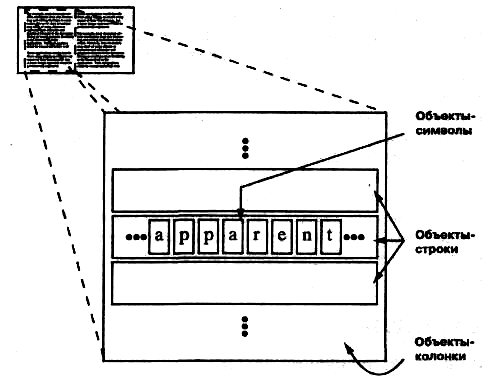
\includegraphics[width=150mm,height=92mm]{pic/text_processor_objs}
  \caption{Использование объектов для представления символов в редакторе документов}
  \label{pic:text_processor_objs}
\end{figure}

У такого дизайна есть один недостаток --- стоимость.
Даже в документе скромных размеров было бы несколько сотен тысяч объектов-символов,
а это привело бы к расходованию огромного объема памяти и неприемлемым затратам во время
выполнения. Паттерн приспособленец показывает, как разделять очень мелкие
объекты без недопустимо высоких издержек.

Приспособленец --- это разделяемый объект, который можно использовать
одновременно в нескольких контекстах. В каждом контексте он выглядит как
независимый объект, то есть неотличим от экземпляра, который не разделяется.
Приспособленцы не могут делать предположений о контексте, в котором работают.

Различные способы хранения глифов символов представлены на рисунке~\ref{pic:sym_storage_schemes}. 

Приспособленцы моделируют концепции или сущности, число которых
слишком велико для представления объектами.
Например, редактор документов мог бы создать по одному приспособленцу для
каждой буквы алфавита. Каждый приспособленец хранит код символа, но координаты
положения символа в документе и стиль его начертания определяются алгоритмами
размещения текста и командами форматирования, действующими в том месте,
где символ появляется. Код символа --- это внутреннее состояние, а все остальное --- внешнее.

Логически для каждого вхождения данного символа в документ существует
объект.

Физически, однако, есть лишь по одному объекту-приспособленцу для каждого
символа, который появляется в различных контекстах в структуре документа.
Каждое вхождение данного объекта-символа ссылается на один и тот же экземпляр в
разделяемом пуле объектов-приспособленцев.

\begin{figure}[htbp]
  \centering
  \begin{subfigure}[b]{\textwidth}
    \centering
    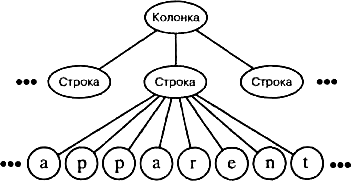
\includegraphics[width=150mm,height=62mm]{pic/text_objs_repr}
    \caption{Использование объектов для хранения каждого символа}
    \label{pic:sym_storage_objs}
  \end{subfigure}

  \bigskip
  
  \begin{subfigure}[b]{\textwidth}
    \centering
    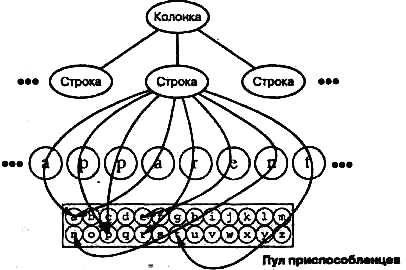
\includegraphics[width=150mm,height=92mm]{pic/text_fly_repr}
    \caption{Использование паттерна <<приспособленец>> для хранения символов}
    \label{pic:sym_storage_fly}
  \end{subfigure}
  \caption{Способы хранения глифов символов в редакторе документов}
  \label{pic:sym_storage_schemes}
\end{figure}

На рисунке~\ref{pic:glyph_uml} изображена структура класса для этих объектов.
Glyph --- это абстрактный класс для представления графических объектов
(некоторые из них могут быть приспособленцами).
Операции, которые могут зависеть от внешнего состояния, передают его в качестве параметра.
Например, операциям Draw (рисование) и Intersects (пересечение) должно быть известно,
в каком контексте встречается глиф, иначе они не смогут выполнить то, что от них требуется.

\begin{figure}[htbp]
  \centering
  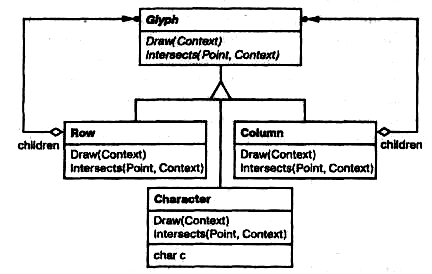
\includegraphics[width=150mm,height=92mm]{pic/glyph_uml}
  \caption{Использование объектов для представления символов в редакторе документов}
  \label{pic:glyph_uml}
\end{figure}

Приспособленец, представляющий букву «а», содержит только соответствующий ей код;
ни положение, ни шрифт буквы ему хранить не надо.
Клиенты передают приспособленцу всю зависящую от контекста информацию, которая нужна,
чтобы он мог изобразить себя. Например, глифу Row известно, где его потомки
должны себя показать, чтобы это выглядело как горизонтальная строка. Поэтому
вместе с запросом на рисование он может передавать каждому потомку координаты.

Поскольку число различных объектов-символов гораздо меньше, чем число
символов в документе, то и общее количество объектов существенно меньше, чем
было бы при простой реализации. 
Документ, в котором все символы изображаются одним шрифтом и цветом,
создаст порядка 100 объектов-символов (это примерно равно числу кодов в таблице ASCII)
независимо от своего размера. А поскольку в большинстве документов применяется
не более десятка различных комбинаций шрифта и цвета, то на практике эта величина
возрастет несущественно. Поэтому абстракция объекта становится применимой и к отдельным символам.

\subsection{Применимость}

Паттерн <<приспособленец>> следует применять в тех случаях,
когда выполняются все нижеперечисленные условия:

\begin{itemize}
\item в приложении используется большое число объектов;

\item из-за этого накладные расходы на хранение высоки;

\item большую часть состояния объектов можно вынести вовне;

\item многие группы объектов можно заменить относительно небольшим количе-
ством разделяемых объектов, поскольку внешнее состояние вынесено;

\item приложение не зависит от идентичности объекта. 
\end{itemize}

\subsection{Структура}

Структура паттерна проектирования <<приспособленец>> приведена
на рисунке~\ref{pic:fly_scheme}. Рассмотрим классы, участвующие в паттерне.

\textbf{Flyweight} (Glyph) --- приспособленец:
объявляет интерфейс, с помощью которого приспособленцы могут получать
внешнее состояние или как-то воздействовать на него.

\textbf{ConcreteFlyweight} (Character) --- конкретный приспособленец:
реализует интерфейс класса Flyweight и добавляет при необходимости
внутреннее состояние. Объект класса ConcreteFlyweight должен быть
разделяемым. Любое сохраняемое им состояние должно быть внутренним,
то есть не зависящим от контекста.

\textbf{UnsharedConcreteFlyweight} (Row, Column) --- неразделяемый конкретный приспособленец:
не все подклассы Flyweight обязательно должны быть разделяемыми.
Интерфейс Flyweight допускает разделение, но не навязывает его.
Часто у объектов UnsharedConcreteFlyweight на некотором уровне структуры
приспособленца есть потомки в виде объектов класса ConcreteFlyweight,
как, например, у объектов классов Row и Column.

\textbf{FlyweightFactory} --- фабрика приспособленцев:
\begin{itemize}
\item Cоздает объекты-приспособленцы и управляет ими.
\item Обеспечивает должное разделение приспособленцев.
  Когда клиент запрашивает приспособленца, объект FlyweightFactory предоставляет
  существующий экземпляр или создает новый, если готового еще нет.
\end{itemize}

\textbf{Client} --- клиент:
\begin{itemize}
\item Хранит ссылки на одного или нескольких приспособленцев.
\item Вычисляет или хранит внешнее состояние приспособленцев.
\end{itemize}

Отношения между классами-участниками:
\begin{itemize}
\item Состояние, необходимое приспособленцу для нормальной работы, можно
  охарактеризовать как внутреннее или внешнее.
  Первое хранится в самом объекте ConcreteFlyweight.
  Внешнее состояние хранится или вычисляется клиентами.
  Клиент передает его приспособленцу при вызове операций.
\item Клиенты не должны создавать экземпляры класса ConcreteFlyweight
  напрямую, а могут получать их только от объекта FlyweightFactory. Это
  позволит гарантировать корректное разделение.
\end{itemize}

\begin{figure}[htbp]
  \centering
  \begin{subfigure}[b]{\textwidth}
    \centering
    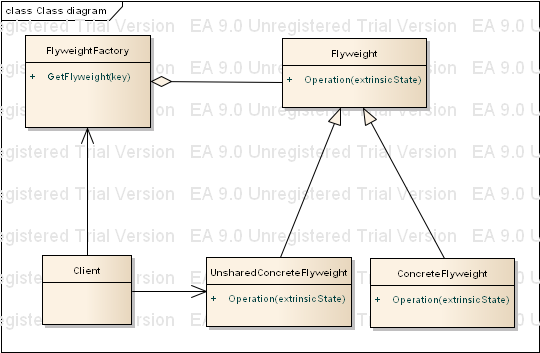
\includegraphics[width=150mm,height=92mm]{pic/flyweight_uml}
    \caption{Диаграмма классов паттерна <<приспособленец>>}
    \label{pic:fly_uml}
  \end{subfigure}

  \bigskip
  
  \begin{subfigure}[b]{\textwidth}
    \centering
    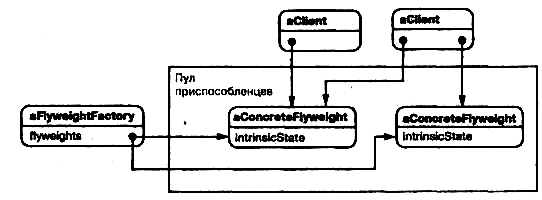
\includegraphics[width=150mm,height=62mm]{pic/flyweight_usage}
    \caption{Схема использования паттерна <<приспособленец>>}
    \label{pic:fly_usage}
  \end{subfigure}
  \caption{Структура паттерна проектирования <<приспособленец>>}
  \label{pic:fly_scheme}

\end{figure}


\subsection{Результаты использования паттерна}

При использовании приспособленцев не исключены затраты на передачу,
поиск или вычисление внутреннего состояния, особенно если раньше оно хранилось
как внутреннее.
Однако такие расходы с лихвой компенсируются экономией памяти за счет разделения 
объектов-приспособленцев.
Экономия памяти возникает по ряду причин:
\begin{itemize}
\item уменьшение общего числа экземпляров;
\item сокращение объема памяти, необходимого для хранения внутреннего состояния;
\item вычисление, а не хранение внешнего состояния (если это действительно так).
\end{itemize}

Чем выше степень разделения приспособленцев, тем существеннее экономия.
С увеличением объема разделяемого состояния экономия также возрастает.
Самого большого эффекта удается добиться, когда суммарный объем внутренней
и внешней информации о состоянии велик, а внешнее состояние вычисляется, а не
хранится. Тогда разделение уменьшает стоимость хранения внутреннего состояния,
а за счет вычислений сокращается память, отводимая под внешнее состояние.

\subsection{Реализация}

При реализации приспособленца следует обратить внимание на следующие
вопросы:
\begin{itemize}
\item
  Вынесение внешнего состояния. 
  Применимость паттерна в значительной степени зависит от того,
  насколько легко идентифицировать внешнее состояние и вынести его за
  пределы разделяемых объектов. Вынесение внешнего состояния не уменьшает
  стоимости хранения, если различных внешних состояний так же много,
  как и объектов до разделения. Лучший вариант --- внешнее состояние
  вычисляется по объектам с другой структурой, требующей значительно меньшей памяти.

\item
  Управление разделяемыми объектами. Так как объекты разделяются, 
  клиенты не должны инстанцировать их напрямую. Фабрика FlyweightFactory
  позволяет клиентам найти подходящего приспособленца. В объектах этого
  класса часто есть хранилище, организованное в виде ассоциативного массива,
  с помощью которого можно быстро находить приспособленца, нужного
  клиенту. 
  Разделяемость подразумевает также, что имеется некоторая форма подсчета
  ссылок или сбора мусора для освобождения занимаемой приспособленцем
  памяти, когда необходимость в нем отпадает. Однако ни то, ни другое
  необязательно, если число приспособленцев фиксировано и невелико (например,
  если речь идет о представлении набора символов кода ASCII).
  В таком случае имеет смысл хранить приспособленцев постоянно.
\end{itemize}

\subsection{Пример использования}

Возвращаясь к примеру с редактором документов, определим базовый класс
Glyph для графических объектов-приспособленцев.
Логически глифы --- это составные объекты, которые обладают графическими
атрибутами и умеют изображать себя. Определение классов Glyph и Character приведено на рисунке~\ref{lst:Glyph_Character} 

\begin{lstlisting}[float,language=c++,caption=Классы Glyph и Character,label=lst:Glyph_Character]
class Glyph {
  public:
    virtual ~Glyph();
    virtual void Draw(Window*, GlyphContext&);
    virtual void SetFont(Font*, GlyphContext&);
    virtual Font* GetFont(GlyphContext&);
    virtual void First(GlyphContext&);
    virtual void Next(GlyphContext&);
    virtual bool IsDone(GlyphContext&);
    virtual Glyph* Current(GlyphContext&);
    virtual void Insert(Glyph*, GlyphContext&);
    virtual void Remove(GlyphContext&};
  protected:
    Glyph();
};

class Character : public Glyph {
  public:
    Character(char);
    virtual void Draw(Window*, GlyphContext\&);
  private:
    char _charcode;
};
\end{lstlisting}

Чтобы не выделять память для шрифта каждого глифа, будем хранить этот
атрибут во внешнем объекте класса GlyphContext, приведенный на рисунке~\ref{lst:GlyphContext}.
Данный объект поддерживает соответствие между глифом и его шрифтом
(а также любыми другими графическими атрибутами) в различных контекстах.
Любой операции, у которой должна быть информация о шрифте глифа в данном контексте, 
в качестве параметра будет передаваться экземпляр GlyphContext.
У него операция и может запросить нужные сведения. Контекст определяется положением глифа в структуре.
Поэтому операциями обхода и манипулирования потомками обновляется GlyphContext

\begin{lstlisting}[float,language=c++,caption=Класс GlyphContext,label=lst:GlyphContext]
class GlyphContext {
  public:
    GlyphContext();
    virtual -GlyphContext();
    virtual void Next(int step = 1);
    virtual void Insert(int quantity = 1);
    virtual Font* GetFont();
    virtual void SetFont(Font*, int span = 1);
  private:
    int _index;
    BTree* _fonts;
};
\end{lstlisting}

Объекту GlyphContext должно быть известно о текущем положении в структуре
глифов во время ее обхода. Операция GlyphContext::Next увеличивает
переменную \_index по мере обхода структуры.
Подклассы класса Glyph, имеющие потомков (например, Row и Column),
должны реализовывать операцию Next так, чтобы она вызывала
GlyphContext::Next в каждой точке обхода.

Операция GlyphContext::GetFont использует переменную \_index в качестве
ключа для структуры ВТгее, в которой хранится отображение между глифами
и шрифтами. Каждый узел дерева помечен длиной строки, для которой он
предоставляет информацию о шрифте. Листья дерева указывают на шрифт, а внутренние
узлы разбивают строку на подстроки - по одной для каждого потомка.


И наконец, нам нужна еще фабрика FlyweightFactory, которая создает глифы и
обеспечивает их корректное разделение. Класс GlyphFactory, представленный 
на рисунке~\ref{lst:GlyphFactory} создает объекты Character и глифы других видов.
Разделению подлежат только объекты Character.
Составных глифов гораздо больше, и их существенное состояние
(то есть множество потомков) в любом случае является внутренним.

\begin{lstlisting}[float,language=c++,caption=Класс GlyphFactory,label=lst:GlyphFactory]
const int NCHARCODES = 128;

class GlyphFactory {
  public:
    GlyphFactory ();
    virtual ~GlyphFactory ();
    virtual Character* CreateCharacter (char);
    virtual Row* CreateRow();
    virtual Column* CreateColumn();
    // ...
  private:
    Character* _character [NCHARCODES];
};

GlyphFactory::GlyphFactory () {
  for (int i = 0; i < NCHARCODES;
    _character [i] = 0;
}

Character* GlyphFactory::CreateCharacter(char c) {
  if (!_character[c]) {
    _character[c] = new Character(c);
  }
  return _character[c];
}

Row* GlyphFactory::CreateRow () {
  return new Row;
}

Column* GlyphFactory::CreateColumn () {
  return new Column;
}
\end{lstlisting}

Массив \_character содержит указатели на глифы Character, индексированные
кодом символа. Конструктор инициализирует этот массив нулями.

Операция CreateCharacter ищет символ в массиве и возвращает соответствующий
глиф, если он существует. В противном случае CreateCharacter создает глиф,
помещает его в массив и затем возвращает.

Остальные операции просто создают новый объект при каждом обращении,
так как несимвольные глифы не разделяются. Эти операции можно было бы опустить
и позволить клиентам инстанцировать неразделяемые глифы напрямую.
Но если позже мы решим сделать разделяемыми и их тоже,
то придется изменять клиентский код, в котором они создаются.

Материалы для ответа взяты из источника~\cite{gamma01}.